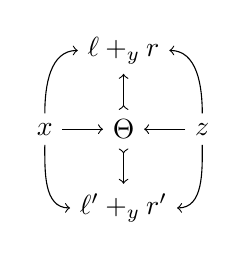
\begin{tikzpicture}
\node [->] (v1) at (-1,0) {$x$};
\node [->] (v3) at (0,1) {$\ell +_y r$};
\node [->] (v4) at (0,0) {$\Theta$};
\node [->] (v5) at (0,-1) {$\ell' +_y r'$};
\node [->] (v7) at (1,0) {$z$};
%
\draw [->]  (v1) edge [out=90,in=180] (v3);
\draw [->]  (v1) edge (v4);
\draw [->]  (v1) edge [out=-90,in=180] (v5);
\draw [->] (v7) edge [out=90,in=0] (v3);
\draw [->] (v7) edge (v4);
\draw [->]  (v7) edge [out=-90,in=0] (v5);
\draw [>->] (v4) edge (v3);
\draw [>->] (v4) edge (v5);
\end{tikzpicture}